\chapter{Implementation}\label{chap:Implementation}
This project was conducted in \textit{two} major phases:
\begin{enumerate}
\item I constructed a core mathematical theory for \textit{type slicing} and \textit{cast slicing} formalising what these ideas actually were and considered the changes to the system presented by Seidel et al. for the \textit{type error witnesses search procedure} to work in Hazel.  

\item I implemented the theories, making it suitable for implementation and extending it to the majority of the Hazel language. Further, suitable deviations from the theory, made upon critical evaluation, are detailed throughout.
\end{enumerate}

\section{Type Slicing Theory}\label{sec:TypeSlicingTheory}

I develop a novel method, \textit{type slicing}, as a mechanism to aid programmers in understanding \textit{why} a term has a given type via static means. Three slicing mechanism have been devised with differing characteristics, all of which associate terms with their typing derivation to produce a \textit{typing slices}. 

The first two criteria attempt to give insight on the structure of the typing derivations, and hence how types are decided. While the third criterion gives a complete picture of the regions of code which contribute to the a term's type.

I would like to stress that the second and third criterion were \textit{very challenging} to formalise, requiring non-obvious mathematical machinery: \textit{context typing slices} (\cref{sec:ContextTypingSlices}), \textit{checking contexts} (\cref{def:CheckingContext}), and \textit{type-indexed slices} (\cref{sec:TypeIndexedSlices}).

\subsection{Expression Typing Slices}\label{sec:ExpressionTypingSlices}
First, I introduce what \textit{slices} are in this context. The aim is to provide a formal representation of term \textit{highlighting}. 

\subsubsection{Term Slices}
A \textit{term slice} is a term with some sub-terms omitted. The omitted terms are those that are \textit{not} highlighted. For example if my slicing criterion is to \textit{omit terms which are typed as} \code{Int}, then the following expressions highlights as:

\[\hlcmaths[yellow!30]{(\lambda x: \code{Int}.\ \lambda y : \code{Bool}.}\ x\hlcmaths[yellow!30]{)(}1\hlcmaths[yellow!30]{)}\]


Omitted sub-terms are replaced by a \textit{gap} term, notated $\gap$. Representing the highlighted example above, we get the slice:
\[(\lambda x : \code{Int}.\ \lambda y : \code{Bool}.\ \gap)(\gap)\]

Similarly, this one can omit variable names and parts of types. We get a syntax specified in \cref{def:ExpressionSliceSyntax}, extending the Hazel core syntax from \cref{fig:syntax}: 
\begin{definition}[Term Slice Syntax]
\label{def:ExpressionSliceSyntax}
Pattern expression slices $p$:
\[p ::= \gap \mid x\]
Type slices $\upsilon$:\footnote{A \textit{type slice} is also used to refer to this whole mechanism. The overall theory is referred to \textit{typing slices} to distinguish from slices of type terms where ambiguous.}
\[\upsilon ::= \gap \mid \dyn \mid b \mid \upsilon \to \upsilon\]
Expression slices $\varsigma$:
\[\varsigma ::= \gap \mid  c \mid x \mid \lambda p : \upsilon.\ \varsigma \mid \lambda p.\ \varsigma \mid \varsigma(\varsigma) \mid \hole^u \mid \hole[\varsigma]^u \mid \varsigma : \upsilon\]
\end{definition}

We then have a \textit{precision} relation on term slices: $\varsigma_1 \sqsubseteq \varsigma_2$ meaning $\varsigma_1$ is less or equally precise than $\varsigma_2$. That is, $\varsigma_1$ matches $\varsigma_2$ structurally except that some sub-terms may be gaps. Full definition in appendix \textbf{ref appendix}. For example, see this precision chain:
\[\gap \sqsubseteq\gap + \gap\sqsubseteq 1 + \gap \sqsubseteq 1 + 2\]
Precision forms a partial order \cite{PartialOrder}, that is, a reflexive, antisymmetric, and transitive relation. Respectively:
\[\inference{}{\varsigma \sqsubseteq \varsigma} \quad \inference{\varsigma_1 \sqsubseteq \varsigma_2 & \varsigma_2 \sqsubseteq \varsigma_1}{\varsigma_1 = \varsigma_2} \quad \inference{\varsigma_1 \sqsubseteq \varsigma_2 & \varsigma_2 \sqsubseteq \varsigma_3}{\varsigma_1 \sqsubseteq \varsigma_3}\]
We also have a \textit{bottom} (least) element, $\gap \sqsubseteq \varsigma$ (for all $\varsigma$). This relation is trivially extended to include \textit{complete terms}\footnote{With no gaps.} $e$ which are \textit{top} elements of their respective chains: if $e \sqsubseteq \varsigma$ then $e = \varsigma$. Sometimes I refer to this relation as $\varsigma_1$ is a term slice \textit{of} $\varsigma_2$ iff $\varsigma_1 \sqsubseteq \varsigma_2$.


\paragraph{Lattice Structure:}\label{sec:JoinTypesTheory} For any \textit{complete term} $t$, the slices of $t$ form a \textit{bounded lattice structure} \cite{Lattice}. That is, every pair $\varsigma_1, \varsigma_2$ has a \textit{join} $\varsigma_1 \sqcup \varsigma_2$ and \textit{meet} $\varsigma_1 \sqcap \varsigma_2$. Full details on this are found in the appendix. Note that not every pair of slices has a join: consider $1$ and $2$. But, every pair does have a meet as for all $\varsigma_1, \varsigma_2$, $\gap \sqsubseteq \varsigma_1$ and $\gap \sqsubseteq \varsigma_2$.
 
\subsubsection{Typing Assumption Slices}
Expression typing is performed given a set of \textit{typing assumptions}. Therefore, in addition to a slice of expressions, we also desire a slice of the typing assumptions, to represent the \textit{relevant}\footnote{Relevant to the given criterion.} parts of the typing assumptions. Typing assumptions are \textit{partial functions} mapping variables to types notated $x : \tau$ (see \cref{sec:TypingJudgements}). 

\textit{Typing assumptions slices} can be represented by partial functions mapping variables to \textit{type slices}. That is, a typing assumption set is a slice of another if it maps \textit{no more} variables to \textit{at most} as specific types. The precision relation, $\sqsubseteq$, can be extended to typing assumptions by extensionality \cite{Extensionality} and using the subset relation:

\begin{definition}[Typing Assumption Slice Precision]
For typing assumption slices $\gamma_1, \gamma_2$. Where $\mathrm{dom}(f)$ is the set of variables for which a partial function $f$ is \textit{defined}:
\[\gamma_1 \sqsubseteq \gamma_2 \iff \mathrm{dom}(\gamma_1) \subseteq \mathrm{dom}(\gamma_2) \text{ and } \forall x \in  \mathrm{dom}(\gamma_1).\ \gamma_1(x) \sqsubseteq \gamma_2(x)\]
\end{definition}
Equally, joins and meet can be extended extensionality:
\begin{definition}[Typing Assumption Slice Joins and Meets]
For typing slices $\gamma_1, \gamma_2$, and any variable $x$: If $\gamma_1(x) = \bot$ then $(\gamma_1 \sqcup \gamma_2)(x) = \gamma_2(x)$ and $(\gamma_1 \sqcap \gamma_2)(x) = \bot$, analogously if $\gamma_2(x) = \bot$. Otherwise, $(\gamma_1 \sqcup \gamma_2)(x) = \gamma_1(x) \sqcup \gamma_2(x)$.
\end{definition}
Again, the slices $\gamma$ of complete typing assumptions $\Gamma$ form a bounded lattice. Again, not every pair of slices has a join, as not every type slice has a join: consider $x : \code{Int}$ and $x : \code{String}$.

\subsubsection{Expression Typing Slices}
Finally, an \textit{expression typing slice}, $\rho$, is a pair, $\varsigma^\gamma$, of a term slice and a typing slice. Precision, joins and meets, can be extended pointwise to term typing slices with all the same properties:
\begin{definition}[Expression Typing Slice Precision]
For expression typing slices $\varsigma_1^{\gamma_1}$, $\varsigma_2^{\gamma_2}$:
\[\varsigma_1^{\gamma_1} \sqsubseteq \varsigma_2^{\gamma_2} \iff  \varsigma_1 \sqsubseteq \varsigma_2 \text{ and } \gamma_1 \sqsubseteq \gamma_2\]
\end{definition}
\begin{definition}[Expression Typing Slice Joins and Meets]
For expression typing slices $\varsigma_1^{\gamma_1}$, $\varsigma_2^{\gamma_2}$:
\[\varsigma_1^{\gamma_1} \sqcup \varsigma_2^{\gamma_2} = (\varsigma_1 \sqcup \varsigma_2)^{\gamma_1 \sqcup \gamma_2}\]
\[\varsigma_1^{\gamma_1} \sqcap \varsigma_2^{\gamma_2} = (\varsigma_1 \sqcap \varsigma_2)^{\gamma_1 \sqcap \gamma_2}\]
\end{definition}

For any pair of complete expressions $e$ and typing assumptions $\Gamma$, then the expression typing slices of these forms a bounded lattice.

\paragraph{Typing Checking:} The \textit{expression slices} can be \textit{type checked} under the \textit{type assumption slices} by replacing gaps $\gap$ by: holes of arbitrary metavariable $\hole^u$ in \textit{expressions}, fresh variables in \textit{patterns}, and the dynamic type in \textit{types}. $\type{\cdot}$ is stated formally in the appendix.

\begin{definition}[Expression Typing Slice Type Checking]
For expression typing slice $\varsigma^{\gamma}$ and type $\tau$. $\synthesis[\gamma]{\varsigma}{\tau}$ iff $\synthesis[\type{\gamma}]{\type{\varsigma}}{\tau}$ and $\analysis[\gamma]{\varsigma}{\tau}$ iff $\analysis[\type{\gamma}]{\type{\varsigma}}{\tau}$.
\end{definition}
\subsection{Context Typing Slices}\label{sec:ContextTypingSlices}
Next, some of an expression's type might be enforced by the surrounding \textit{context}. For example, the  type of the underlined expression below is enforced by the surrounding highlighted annotation:
\[\underline{(\lambda x. \hole^u )} \hlcmaths[yellow!30]{:  \code{Bool} \hlcmaths[yellow!30]{\to \code{Int}}}\]

\subsubsection{Contexts \& Context Slices}
\renewcommand{\C}{\mathdcal{C}}
We represent these surrounding contexts by a \textit{term context} $\mathdcal{C}$. Which marks \textit{exactly one} sub-term as $\cmark$:
\begin{definition}[Contexts Syntax]
Pattern contexts -- mapping patterns to patterns:
\[\mathdcal{P} ::= \cmark\]
Type contexts -- mapping types to types: 
\[\mathdcal{T} ::= \cmark \mid \mathdcal{T} \to \tau \mid \tau \to \mathdcal{T}\]
Expression contexts -- mapping patterns, types, or expression to expressions:\footnote{Note that $\C$ is also used for generic term contexts sometimes.}
\[\C ::=  \cmark \mid \lambda \mathdcal{P} : \tau.\ e \mid \lambda x : \mathdcal{T}.\ e \mid \lambda x : \tau.\ \C \mid \lambda \mathdcal{P}.\ e \mid \lambda x.\ \C \mid \C(e) \mid e(\C) \mid e : \mathdcal{T} \mid \C : \tau\]
\end{definition}

Where $\C\{e\}$ substitutes expression $e$ for the mark $\cmark$ in $\C$, the result of this is necessarily an expression. Similarly for pattern and type contexts $\mathdcal{P}, \mathdcal{T}$ whose substitutions return patterns and types. Additionally, contexts are \textit{composable}: substituting a context into a context, $\C_1\{\C_2\}$ produces another valid context when the domain of $\C_1$ is from expressions. Notate this by $\C_1 \circ \C_2$. From here on I notate all contexts like functions, specifying their domain and co-domain where appropriate: $\C : \code{Typ} \to \code{Exp}$ for example.


\newcommand{\Cs}{\mathdcal{c}}
\newcommand{\p}{\mathdcal{p}}
Then, contexts can be extended to slices, $\Cs$, analogously to the previous section. However, the precision relation $\sqsubseteq$ is defined differently, requiring that the mark $\cmark$ must remain in the same position in the structure. For example $\cmark(\gap) \sqsubseteq \cmark(1)$, but $\cmark \not \sqsubseteq \cmark(1)$. This can be concisely defined by \textit{extensionality}:

\begin{definition}[Context Precision]\label{def:ContextPrecision}
If $\Cs : \code{X} \to \code{Y}$ and $\Cs' : \code{X} \to \code{Y}$ are context slices, then $\Cs' \sqsubseteq \Cs$ if and only if, for all terms $t$ of class $\code{X}$, that $\Cs'\{t\} \sqsubseteq \Cs\{t\}$.
\end{definition}

Again, we refer to a context slice $\Cs'$ \textit{of} $\Cs$ as one satisfying that $\Cs' \sqsubseteq \Cs$.

We also get that filling contexts preserves the precision relations both on term slices \textit{and} context slices:\footnote{The conjectures are heavily suspected but not formally proven yet.}
\begin{conjecture}[Context Filling Preserves Precision]
For context slice $\Cs : \code{X} \to \code{Y}$ and term slice $\varsigma$ of class \code{X}. Then if we have slices $\varsigma' \sqsubseteq \varsigma$, $\Cs' \sqsubseteq \Cs$ then also $\Cs'\{\varsigma'\} \sqsubseteq \Cs\{\varsigma\}$.
\end{conjecture}

Joins and meets can be defined via extensionality as before, and we can still form bounded lattices.

\subsubsection{Typing Assumption Contexts \& Context Slices}
The accompanying notion of a \textit{typing assumption slice} can be extended to \textit{functions on typing assumptions}. This function represents what typing assumptions need to be \textit{added}, or can be \textit{removed} when typing an expression $e$ and within it's context slice.

\renewcommand{\F}{\mathdcal{F}}
\newcommand{\f}{\mathdcal{f}}
\begin{definition}[Typing Assumption Contexts \& Slices]
A typing assumption context $\F$ is a function from typing assumption to typing assumptions. A typing assumption context slice $\f$ is a function from typing assumption slices to typing assumption slices.
\end{definition}

Functions can be composed and a precision partial order can also be defined via extensionality:
\begin{definition}[Typing Assumption Context Slice Precision]\label{def:FunctionPrecision}
If $\f'$ and $\f$ are typing assumption context slices, then $\f' \sqsubseteq \f$ if and only if, for all typing context slices $\gamma$, that $\f'(\gamma) \sqsubseteq \f(\gamma)$.
\end{definition}
Again, such functions are monotone:
\begin{conjecture}[Function Application Preserves Precision]
For typing assumption slice $\gamma$ and typing assumption context slice $\f$. Then if we have slices $\gamma' \sqsubseteq \gamma$, $f' \sqsubseteq f$ then also $f'(\gamma') \sqsubseteq f(\gamma)$.
\end{conjecture}
Joins and meets are also defined extensionally:
\begin{definition}[Typing Assumption Context Slice Joins \& Meets] For typing assumption context slices $\f_1$ and $\f_2$ and any typing assumption slice $\gamma$:
\[(\f_1 \sqcup \f_2)(\gamma) = \f_1(\gamma) \sqcup \f_2(\gamma)\]
\[(\f_1 \sqcap \f_2)(\gamma) = \f_1(\gamma) \sqcap \f_2(\gamma)\]
\end{definition}

\begin{conjecture}[Typing Assumption Context Slices form Bounded Lattices]
For any typing assumption context $\F$, the set of slices $\f$ of $\F$ form a bounded lattice with bottom element being the constant function to the empty typing assumptions and top element $\F$.
\end{conjecture}

As usual, not all joins exist: if the assumption context slices map the slices to inconsistent typing assumption slices. 
\subsubsection{Context Typing Slices}
Finally, an \textit{expression context typing slice}, $\p$, is a pair, $\Cs^\f$, of an expression context slice and a typing assumption context slice. Precision, application, joins and meets, can be extended pointwise as before to term typing slices with all the same properties. The only new extension being of composition and application.
\begin{definition}[Expression Context Typing Slice Composition \& Application]
For expression context typing slices $\Cs^{\f}$, $\Cs'^{\f'}$, and expression typing slices $\varsigma^{\gamma}$:
\[\Cs^{\f} \circ \Cs'^{\f'} =  (\Cs \circ \Cs')^{\f \circ \f'}\]
\[\Cs_1^{\f_1}\{\varsigma^{\gamma}\} =  \Cs_1\{\varsigma\}^{\f_1(\gamma)}\]
\end{definition}

\subsection{Type-Indexed Slices}\label{sec:TypeIndexedSlices}
Tagging slices by their type and allowing decomposition into sub-slices for each part of the type is required for \textit{cast slicing} and useful in calculating slices according to \textit{analysis slices} and \textit{contribution slices} criteria. For example consider the same context slice:
\[\underline{(\lambda x. \hole^u )} \hlcmaths[yellow!30]{:  \code{Bool} \hlcmaths[yellow!30]{\to \code{Int}}}\]
This context slice would be tagged with type $\code{Bool} \to \code{Int}$ and the respective sub-slice considering only the return type would omit the \code{Bool} term:
\[\underline{(\lambda x. \hole^u )} \hlcmaths[yellow!30]{:}  \code{Bool} \hlcmaths[yellow!30]{\to \code{Int}}\]

This section will only consider \textit{context slices}, but term slices are type-indexed in exactly the same way, see the appendix.

The main property that we want these indexed-slices to maintain is that a slice can be \textit{reconstructed} from their sub-parts. \textit{Joining} the sub-slices should produce the slice for the entire type. As sub-slices come from different regions of code, we pair sub-slices with contexts which place the two sub-slices inside the same context, making them join-able.

\renewcommand{\S}{\mathdcal{S}}
\renewcommand{\s}{\mathdcal{s}}
\begin{definition}[Type-Indexed Context Typing Slices]
Syntactically defined: 
\[\S ::= \p \mid \p * \S \to \p * \S\] 
With any $\S$ only being valid if it has a full slice. The full slice of $\S$ is notated $\overline{\S}$ and defined recursively:
\[\overline{\p} = \p\]
\[\overline{\p_1 * \S_1 \to \p_2 * \S_2} = \p_1 \circ \overline{\S_1} \sqcup \p_2 \circ \overline{S_2}\]
\end{definition}
Then left \textit{(incremental)} composition and right \textit{(global)} composition can be defined, by composing at the upper type constructor or at the leaves respectively:
\begin{definition}[Type-Indexed Context Typing Slice Composition]
For type-indexed context typing slices $\S$ and $\S'$.  If $\S = \p$ and $\S' = \p'$:\footnote{In shorthand, the overline for a base type slice is often omitted.}
\[\p' \circ \p = \overline{\p'} \circ \overline{\p}\qquad \p \circ \p' = \overline{\p} \circ \overline{\p'}\]
If $\S = \p$ and $\S' = \p_1' * \S_1' \to \p_2' * \S_2'$:\footnote{In shorthand, brackets will be omitted.}
\[S \circ \S' = (\p \circ p_1') * \S_1' \to (\p \circ \p_2') * \S_2'\]
If $\S = \p_1 * \S_1 \to \p_2 * \S_2$:
\[\S \circ \S' = \p_1 * (\S_1 \circ \S') \to \p_2 * (\S_2 \circ \S')\]
\end{definition}

This definition stems from it representing regular context typing slice composition over it's full slices.
\begin{proposition}[Type-Indexed Composition Preserves Full Slice Composition]
For type-indexed slices $\S$ and $\S'$: 
\[\overline{\S \circ \S'} = \overline{\S} \circ \overline{\S'}\]
\end{proposition}


\subsection{Criterion 1: Synthesis Slices}
\label{sec:SynthesisSlices}

The first slicing method aims to concisely explain why an expression \textit{synthesises} a type. It omits all  sub-terms which analyse against a type retrieved from synthesising some other part of the program. For example, the following term synthesises a $\code{Bool} \to \code{Bool}$ type, and the variable $x : \code{Int}$ and argument are irrelevant:

\[\hlcmaths[yellow!30]{(\lambda} x: \code{Int}\hlcmaths[yellow!30]{.\ \lambda y : \code{Bool}.\ y)(}1\hlcmaths[yellow!30]{)}\]

\begin{definition}[Synthesis Slices]
For a synthesising expression, $synthesis{e}{\tau}$. A synthesis slice is an expression typing slice $\varsigma^{\gamma}$ of $e^\Gamma$ which also synthesises $\tau$, that is, $\synthesis[\type{\gamma}]{\type{\varsigma}}{\tau}$.
\end{definition}
\begin{proposition}[Minimum Synthesis Slices]
A minimum synthesis slice of $e^\Gamma$ is a synthesis slice $\rho$ such that any other synthesis slices $\rho'$ are at least as specific, $\rho \sqsubseteq \rho'$. This minimum always uniquely exists.
\end{proposition}

These slices can be defined via a typing judgement $\synthesisslice{e}{\tau}{\S}$, meaning $\S$ is the type-indexed synthesis slice of $e^\Gamma$ synthesising $\tau$. The non-indexed version can be retrieved by $\overline{\S}$. This judgement mimics the Hazel typing rules, while omitting portions of the program which are \textit{type analysed} from the slice.  

For example, when encountering application, the type of the function is synthesised purely by the function itself, so the argument can be omitted:
\[\inference{\synthesisslice{e_1}{\tau_1}{\S_1} & \tau_1 \funmatch \tau_2 \to \tau & \S_1 \funmatch \S_2 \to \S & \analysis{e_2}{\tau_2}}{\synthesisslice{e_1(e_2)}{\tau}{\S}}\]
Where function matching $\funmatch$ is extended to slices by eagerly applying the contexts paired with the slice sub-parts if applicable:
\[\Cs \funmatch \Cs \to \Cs\]
\[\Cs_1 * \S_1 \to \Cs_2 * \S_2 \funmatch \Cs_1 \circ \S_1 \to \Cs_2 \circ \S_2\]
This approach correctly calculates the synthesis slices.
\begin{conjecture}[Correctness]
\label{conj:SynthesisSliceCorrectness}
If $\synthesis{e}{\tau}$ then:
\begin{itemize}
\item $\synthesisslice{e}{\tau}{\rho}$ where $\rho = \varsigma^\gamma$ with $\synthesis[\gamma]{\varsigma}{\tau}$.
\item For any $\rho' = \varsigma'^{\gamma'} \sqsubseteq e^\Gamma$ such that $\synthesis[\gamma']{\varsigma'}{\tau}$ then $\rho \sqsubseteq \rho'$.
\end{itemize}
\end{conjecture}

\subsection{Criterion 2: Analysis Slices}\label{sec:AnalysisSlices}
A similar idea can be devised for type analysis. The way to represent these are \textit{context slices}. After all, it is the terms immediately \textit{around} the sub-term where the type checking is enforced. For example, when checking this annotated term:
\[(\lambda x. \hole^u) : \code{Bool} \to \code{Int}\]
The \textit{inner hole term} $\hole^u$ (underlined) is required to be consistent with \code{Int} due to the annotation. Therefore, the hole's analysis slice will be:
\[\hlcmaths[yellow!30]{(\lambda} x\hlcmaths[yellow!30]{.} \underline{\hole^u} \hlcmaths[yellow!30]{) : } \code{Bool} \hlcmaths[yellow!30]{\to \code{Int}}\]
Intuitively, this means that the \textit{contextual} reason for $\hole^u$ to be required to be an \code{Int} is: that it is within a function which the annotation enforced to check against $\code{Bool} \to \code{Int}$, of which only the return type ($\code{Int}$) is relevant.

In other words, if the context slice was type synthesised, then the marked term would still be \textit{required} to check against \code{Int}. However, the overall synthesised type may differ.\footnote{The previous example would synthesis $\dyn \to \code{Int}$ as opposed to $\code{Bool} \to \code{Int}$.}


\subsubsection{Checking Context}
For this, we only want to consider the smallest context scope\footnote{The \textit{size} of the context around the marked term.} that enforced the type checking. For example, the below term has 3 annotations, but only the inner one enforces the \code{Int} type on the integer 1:
\[\underline{1} \hlcmaths[yellow!30]{: \code{Int}} : \dyn : \code{Bool}\]
I refer to this minimum context scope as the \textit{minimally scoped checking context}; checking contexts will always synthesise a type. To give another example, an integer argument's type is enforced by the annotation on the function:
\[\hlcmaths[yellow!30]{(\lambda} x \hlcmaths[yellow!30]{: \code{Int}.}\ \hole^u\hlcmaths[yellow!30]{)(}\underline{1}\hlcmaths[yellow!30]{)}\]


\begin{definition}[Checking Context]
\label{def:CheckingContext}
For term $e$ checking against $\tau$: $\analysis[\Gamma]{e}{\tau}$. A checking context for $e$ is an expression context $\C$ and typing assumption context $\F$ such that: 
\begin{itemize}
\item $\C \neq \cmark$.
\item $\synthesis[\F(\Gamma)]{\C\{e\}}{\tau'}$ for some $\tau'$.
\item The above derivation has a sub-derivation $\analysis[\Gamma]{e}{\tau}$.
\end{itemize}
\end{definition}
\begin{definition}[Minimally Scoped Checking Context]
For a derivation $\analysis[\Gamma]{e}{\tau}$, a minimally scoped expression checking context is a checking context of $e$ such that no sub-context is also a checking context.
\end{definition}

All possible minimally scoped checking contexts can be constructed syntactically via rules. These coincide with the definition above, but is more amenable to performing proofs on. Given in the appendix \textbf{ref}.

Sub-terms of a program which are analysed will have unique checking contexts that are also part of the program:
\begin{proposition}[Checking Context of a Sub-term in a Derivation]
If derivation $\synthesis{e}{\tau}$ contains a analysis sub-derivation $\analysis[\Gamma']{e'}{\tau'}$ for sub-term $e'$. Then there is a unique minimally scoped context $\C$ for $e'$ and typing assumption context $\F$ for $\Gamma'$ such that:
\begin{itemize}
\item $\C\{e'\}$ is a sub-term of $e$, or is $e$ itself.
\item Derivation $\synthesis{e}{\tau}$ contains a sub-derivation for $\synthesis[\F(\Gamma')]{\C\{e'\}}{\tau''}$, or is the derivation itself: $\tau'' = \tau, \C\{e'\} = e,$ and $\F(\Gamma') = \Gamma$.
\end{itemize}
\end{proposition}

Analysis slices are then a slice of any \textit{minimally scoped checking context}.
\begin{definition}[Analysis Slice]\label{def:analysisslice}
For a term $e$ analysing against $\tau$: $\analysis{e}{\tau}$, and a minimally scoped checking context $\C^\F$ for $e$. An analysis slice is a slice $\Cs^\f$ of $\C^\F$ which is also a checking context for $e$. That is:
\begin{itemize}
\item $\synthesis[\f(\Gamma)]{\Cs\{e\}}{\tau'}$ for some $\tau'$.
\item The above derivation has a sub-derivation for $\analysis{e}{\tau}$. 
\end{itemize}
\end{definition}

The \textit{minimum analysis slice} is just the minimum under the precision ordering $\sqsubseteq$. And it must be unique:

\begin{conjecture}[Minimum Analysis Slices]\label{conj:AnalysisSliceUniqueness}
The minimum analysis slice analysing $e$ in a checking context $\C^\F$ is an analysis slice $\p$ such that for any other any other analysis slice $\p'$ is at least as specific, $\p \sqsubseteq \p'$. This minimum always uniquely exists.
\end{conjecture}

This can again be represented by a judgement read as, \textit{$e$ which type checks against $\tau$ in checking context $\C$ has (type-indexed) analysis slice $\S$}:\footnote{Again, non-indexed version retrieved by $\overline{\S}$.}
\[\analysisslice{\C}{e}{\tau}{\p}\]

There are two situations which enforce \textit{checking contexts}, of which application is most interesting, calculating the minimum indexed synthesis slice of the context and retrieving just the sub-slice relevant to typing the \textit{argument}:\footnote{Note that $e_1$ synthesises $\tau_2$ exactly here. Contribution slices consider situations involving subsumption which may synthesise different but consistent types.}

\[\inference{\synthesisslice{e_1}{\tau_1}{\S_1} & \tau_1 \funmatch \tau_2 \to \tau & \S_1 \funmatch \S_2 \to \S & \analysis{e_2}{\tau_2}}{\analysisslice{e_1(\cmark)}{e_2}{\tau_2}{(\Cs^\gamma \mapsto \Cs(\cmark)^{\gamma_2 \mapsto \gamma \sqcup \gamma_2})\ \$\ S_2}}\]
Where the resulting slice takes sub-slices $\rho$ of $\S_2$ and places them in a context $\rho(\cmark)$. That is, if $\S_2$ represented type $\code{Int} \to \code{Bool}$, the result is a context slice also representing $\code{Int} \to \code{Bool}$ with the context for the \code{Int} part being $\rho(\cmark)$ with $\rho \sqsubseteq e_1$ being the sub-slice of the \code{Int} part of $\S_2$ etc. The appendix defines this operation (and it's converse).

\begin{conjecture}[Correctness]\label{conj:AnalysisSliceCorrectness}
If $\C$ is a checking context for $e$ and $\analysis{e}{\tau}$. Then $\analysisslice{\C}{e}{\tau}{\S}$ and $\S$ is the minimum analysis slice of $e$.
\end{conjecture}

\subsection{Criterion 3: Contribution Slices}
\label{sec:ContributionSlices}
This criterion aims to highlight all regions of code which \textit{contribute} to the given type (either synthesised or analysed). Where \textit{contribute} means that there exists a type that the sub-term could change it's type to to change the type of the overall term (or make it ill-typed). For example in the following term:

\[(\lambda f: \code{Int} \to \dyn.\ f(1))\underline{(\lambda x : \code{Int}.\ x)}\]
The terms which \textit{contribute} to the \textit{underlined} lambda term checking successfully against $\code{Int} \to \dyn$ is everything \textit{except} the $x$ term, plus the annotation enforcing the type. Highlights related to synthesis are in a darker shade:
\[\hlcmaths[yellow!30]{(\lambda} f\hlcmaths[yellow!30]{: \code{Int} \to \dyn}.\ f(1)\hlcmaths[yellow!30]{)}\underline{\hlcmaths[yellow!70]{(\lambda} x \hlcmaths[yellow!70]{: \code{Int}.}\ x\hlcmaths[yellow!70]{)}}\]
Notice that, the only sub-terms which \textit{can} have their type changed without affecting the overall type must be expected to be dynamic. Therefore, this criterion just omits all dynamically annotated regions of the program.\footnote{But does not omit the dynamic annotations themselves.}

These can be calculated by just taking the analysis slice and only the static parts of the synthesis slice.

\section{Cast Slicing Theory}\label{sec:CastSlicingTheory}
Cast slicing propagates type slice information during evaluation, by tagging casts types with type slices. The primary reason in using type-indexed slices to calculate type slices was to allow type-slices to be decomposable during evaluation, while retaining only the code relevant to the part of the type involved in the cast. We therefore change the syntax of casts to $\scast{\S}{\S}$. The updated hazel elaboration and dynamics rules must using slices can be found in the appendix, but are relatively trivial.

\section{Type Slicing Implementation}\label{sec:TypeSlicingImplementation}
Here I detail how the theories above were adapted to produce an implementation for Hazel.
\subsection{Hazel Terms}
\label{sec:HazelTerms}
Hazel represents its abstract syntax tree (AST) in a standard way by creating a mutually recursive algebraic data-type. 

Terms are classified into similar groups as described in the calculus (see \cref{sec:HazelSyntax}), though combining external and internal expressions, and adding patterns and environments:
\begin{itemize}
\item \textbf{Expressions}: The primary encompassing term including: constructors\footnote{The basic language constructs: integers, lists, labelled tuples etc. Also, user-defined constructors via sum types.}, holes, operators, variables, let bindings, functions \& closures, type functions, type aliases, pattern match expressions, casts, explicit fix\footnote{Fixed point combinator for recursion.} expression.
\item \textbf{Types}: Unknown type\footnote{Either dynamic type, or a type hole.}, base types, function types, product types, record types, sum types, type variables, universal types, recursive types.
\item \textbf{Patterns}: Destructuring constructs for bindings, used in functions, match statements, and let bindings, including: Holes, variables (to bind values to), wildcard, constructors, annotations (enforcing type requirements on bound variables). 
\item \textbf{Closure Environments}: a closure mapping variables to their assigned values in it's syntactic context.
\end{itemize}

For example \cref{fig:tupletermstructure} shows a let binding expression whose binding is a tuple pattern (in blue) binding two variables \code{x}, \code{y} annotated with a type (in purple).

\begin{figure}[h]
\center
\includegraphics[width=0.75\textwidth]{Media/Figures/tuple_term_structure}
\caption{Let binding a tuple with a type annotation.}
\label{fig:tupletermstructure}
\end{figure}

Every term (and sub-term) is annotated with an \textit{identifier} (ID, \code{Id.t}) in the AST which refers back to the syntax structure tree. In a sense, this is the equivalent of \textit{code locations}, but Hazel is edited via a structure editor. 
\subsection{Type Slice Data-Type}\label{sec:TypeSliceDataType}

\subsubsection{Expression slices as ASTs}

Directly storing expression slices directly as ASTs is both \textit{space and time inefficient}, even when accounting for the persistence \cite[ch. 2]{PurelyFunctionalDataStructures} of trees in OCaml. 

For highlighting purposes, there is no need to retain the structure (unlike the theory, we do not need to type check the results, instead just assuming correctness). 

\subsubsection{Unstructured Code Slices}
\label{sec:UnstructuredSlices}
With this in mind, I represent slices indirectly by their IDs with an \textit{unstructured} list, referred to now as a \textit{code slice}.

Additionally, this allows more \textit{granular} control over slices, as they need not conform with the structure of expressions, which is taken advantage of in reducing slice sizes \cref{sec:SlicingAnalysis}.

\subsubsection{Type-Indexed Slices}
Cast slicing and contribution slices required \textit{type-indexed} slices. I therefore tag type constructors with slices recursively, i.e.:

\begin{figure}[h]
\begin{minted}[fontsize=\small]{reason}
type typslice_typ_term = 
  | Unknown
  | Arrow(slice_t, slice_t)  // Function type
  | ... // Type constructors
and typslice_term = (typslice_typ_term, code_slice)
and typslice_t = IdTagged.t(slice_term)
\end{minted}
\caption{Initial Type Slice Data-Type}
\end{figure}

However, this did not model the structure of type slices particularly well. Slices are generally incrementally constructed. Synthesis slices build slices from the slices of sub-term, so the list data-type is efficient due to it's persistent nature. However, analysis slices add ids to \textit{all} sub-slices. Hence, analysis slices had \textit{quadratic} space complexity in the depth of the type.

\subsubsection{Incremental Slices}
Therefore, I explicitly represent slices incrementally, with two modes, for synthesis slice parts (termed \textit{incremental slice tags}) and analysis slice parts (termed \textit{global slice tags}).

Instead of tagging an id in an analysis slice to all subslices, we tag it only once as a \textit{global slice}, and \textit{lazily} tag it to sub-slices upon usage. That is, when de-constructing types via function matching etc.

We get the following type:
\begin{minted}[fontsize=\small]{reason}
...
and typslice_empty_term = [
  | `Typ(typ_term)
  | `TypSlice(typslice_typ_term)
]
and typslice_incr_term = [
  | `Typ(typ_term)
  | `TypSlice(typslice_typ_term)
  | `SliceIncr(typslice_typ_term, code_slice)
]
and typslice_term = [
  | `Typ(typ_term)
  | `TypSlice(typslice_typ_term)
  | `SliceIncr(typslice_empty_term)
  | `SliceGlobal(typslice_incr_term, code_slice)
]
and typslice_t = IdTagged.t(typslice_term)
...
\end{minted}

The invariant that a slice has at only one incremental and/or global slice is maintained by splitting into three types (\code{empty_term}, \code{incr_term}, \code{term}). While, regular unsliced types are maintained to provide easier interoperability with the rest of the code-base (and allowing type slicing to be turned off).

\textit{Polymorphic Variants} \cite[ch. 7.4]{RealWorldOCaml}, notated \texttt{[ | ... ]} are used to more conveniently write functions on slices. This is possible due \textit{row polymorphism} \cite{PolymorphicVariants} \cite[ch. 10.8]{ATTAPL} relating the variants by a \textit{structural subtyping} relation \cite{StructuralSubtyping}. We have that ($x :> y$ means $x$ a subtype of $y$): 
\[\code{typslice_empty_term} :> \code{typslice_incr_term} :> \code{typslice_term}\]
Type constructors are either co-variant or contra-variant \cite[ch. 2]{BasicCatTheory} with respect to the subtyping relation. For example, id tagging is covariant, so:
\[\code{IdTagged.t(typslice_incr_term)} :> \code{IdTagged.t(typslice_incr_term) = typslice_t}\] 
Equally, as functions are bifunctors, contravariant in their input and covariant in their output:
\[\code{typslice_incr_term} \to \code{typslice_incr_term} :> \code{typslice_empty_term} \to \code{typslice_term}\]

This function subtyping property significantly reduces work in defining functions on this type as seen below.
\paragraph{Utility Functions}
Functions on slices often only concern the underlying type, e.g. checking if a slice is a \textit{list} type. (\textbf{ref to sec}). In which case it is more convenient write a $\code{typ_term} \to \alpha$ and $\code{typslice_term} \to \alpha$ function directly on the possible empty slice types. 

An \code{apply} function is provided to apply this onto the slice term. See how the bottom two branches can both be passed into the \code{apply} function even though they have different types (but are both sub-types of \code{typslice_term}).  
\begin{minted}[fontsize=\small]{reason}
let rec apply = (f_typ, f_slc, s) =>
  switch (s) {
  | `Typ(ty) => f_typ(ty)
  | `TypSlice(slc) => f_slc(slc)
  | `SliceIncr(s, _) => apply(f_typ, f_slc, s)
  | `SliceGlobal(s, _) => apply(f_typ, f_slc, s)
  }
\end{minted}
Other utility functions include mapping functions, wrapping functions, unpacking functions, matching functions etc.

\subsubsection{Type Slice Joins}
Type joins (\cref{sec:JoinTypesTheory}) are extensively used in the Hazel implementation for \textit{branching statements} and in the theory of contribution slices.

For basic type slices, when the same type information is available from multiple branches, only the right branch is used in the slice. For contribution slices, both must be retained. See how the part of the left branch slice is omitted when already known from the right branch in \cref{fig:TypeJoins} (slices highlighted in green). Note that we still needed some information from the left hand side (the first tuple element).

\begin{figure}[h]
\centering
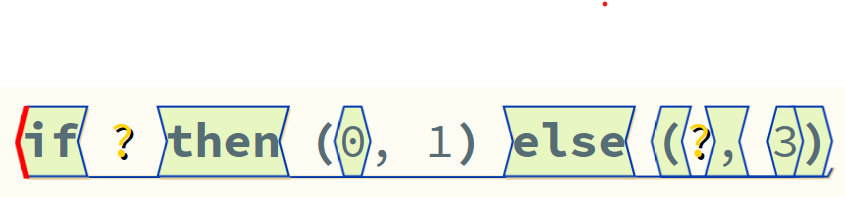
\includegraphics[width=0.5\textwidth]{Media/Figures/typejoin}
\caption{Type Slice Joins}
\label{fig:TypeJoins}
\end{figure}

\subsection{Static Type Checking}\label{sec:TypeChecking}
The Hazel implementation is \textit{bidirectionally typed}. During type checking, the typing \textit{mode} in which to check the term is specified with \code{Mode.t} type: \textit{synthesising}\footnote{Additionally split into synthesising functions and type functions, but this detail is elided here.} (\code{Syn}) or \textit{analysing} (\code{Ana(Typ.t)}).

The type checker associates each term with a type information object \code{Info.t}, stored in a map by term id with efficient access. \code{Info.t} is demonstrated in \cref{fig:Info} with arrows representing dependencies (e.g. a terms type depending on the mode, self, and status).
\begin{figure}[h]
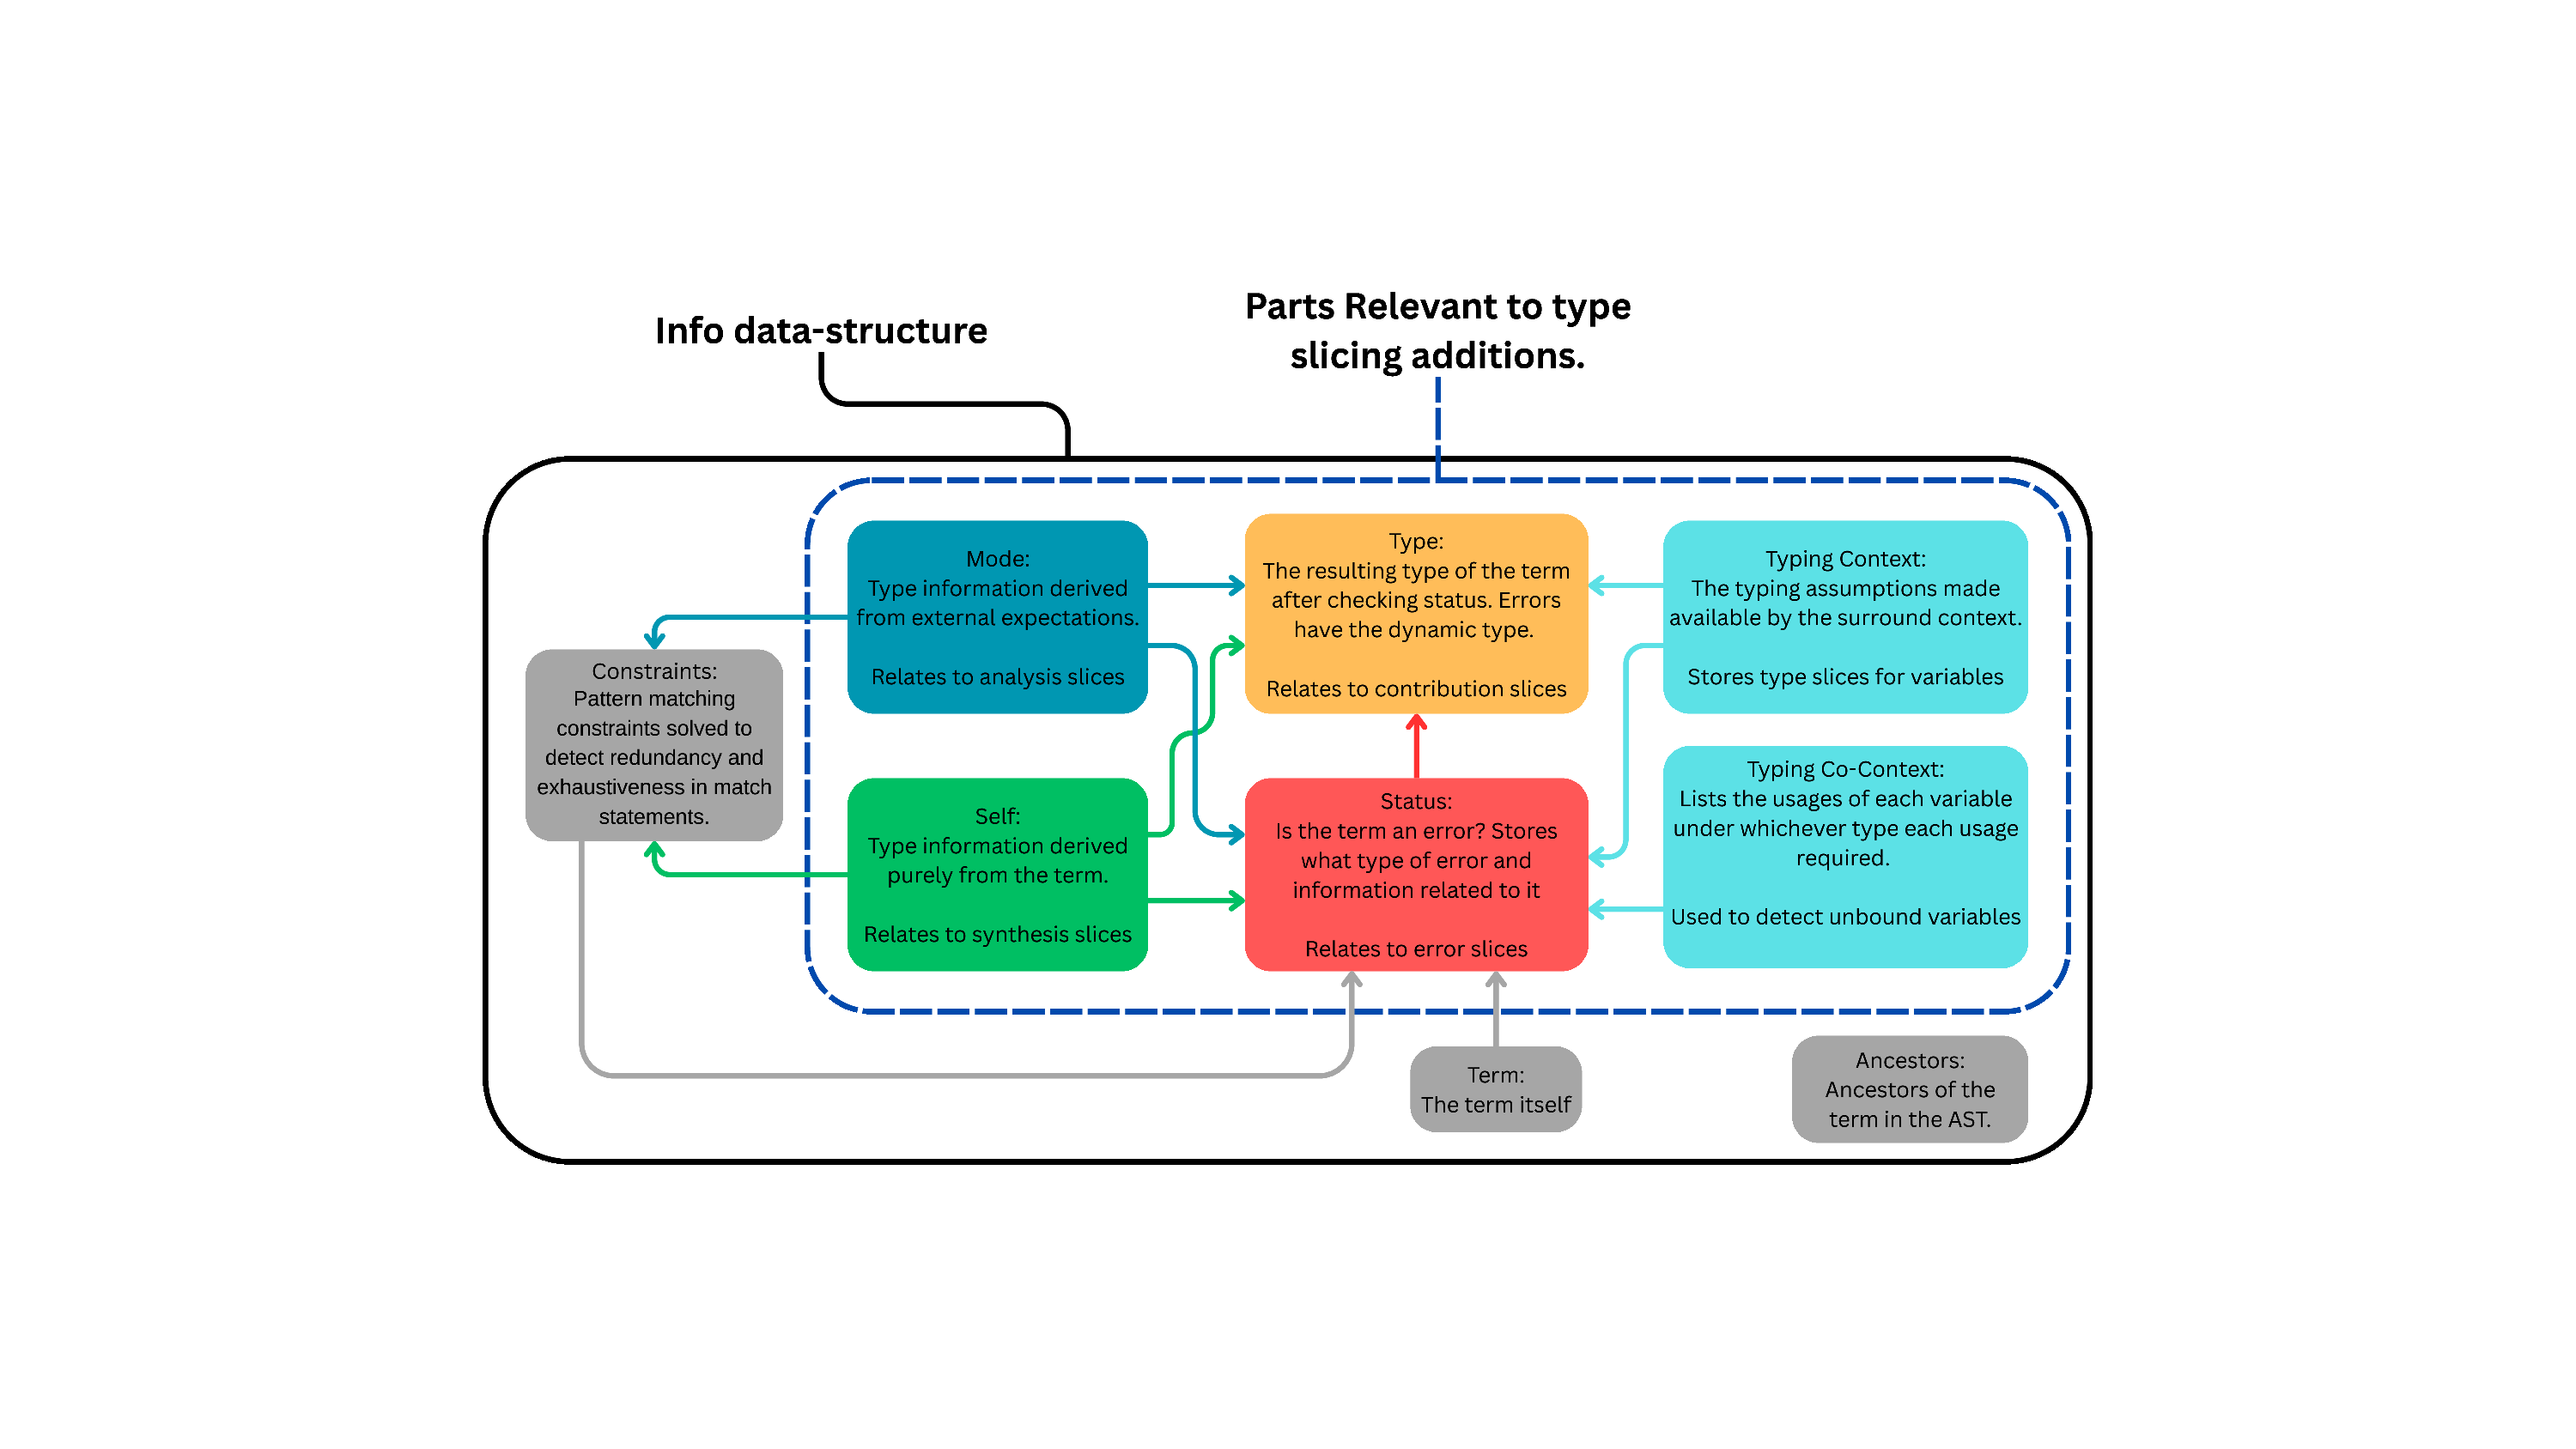
\includegraphics[width=1\textwidth, trim={8cm 5cm 8cm 5cm}, clip]{Media/Figures/info}
\caption{\code{Info.t} data-structure}
\end{figure}

\subsubsection{Self and Mode}
Code relating to synthesis slices and analysis slices is factored into \code{Self.t} and \code{Mode.t}. Additionally, some type checking logic that could be factored but had not yet been on the Hazel dev branch were done so. Despite this, the actual implementation of slicing still requires full knowledge of how the type checker works in order to actually add the \textit{correct} IDs to the slice. Two examples of this slice logic are shown in \cref{sec:slicingstaticsexamples}.

\code{Self.t} uses incremental slices, while \code{Mode.t} uses global slices. These global slices are then retained upon type decomposition (e.g. function matching)..

\subsubsection{Typing (Co-)Context}
The typing context and co-contexts are modified to use type slices. This deviates from the theoretical notion of an expression slice: the structural context in which the variable is used is untracked when passing through the context. Therefore, it requires using \textit{unstructured} code slices. It is a useful addition in practice allowing slices calculated when binding variables to be shown at their use site, see \cref{fig:VarSlice}.
\begin{figure}[h]
\centering
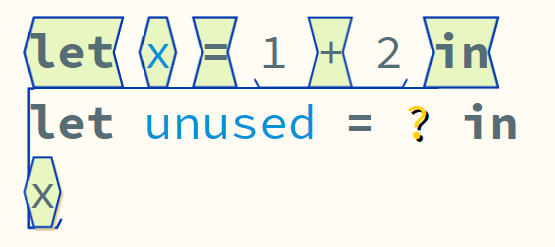
\includegraphics[width=0.3\textwidth]{Media/Figures/var_slice}
\caption{Variable Slice}
\label{fig:VarSlice}
\end{figure}

\subsubsection{Status and Type}
The mode and self are combined to determine the final type. Contribution slices extract the static parts of synthesis slices here. When the synthesised and analysed types are inconsistent, the slice information can be used to construct minimised errors slices (explaining just the inconsistent parts), see \cref{sec:SlicingAnalysis} which demonstrates their retrospective design and effectiveness.

\subsection{Extensions}
To support the full Hazel language, type slices needed to implement many functions, for example: type substitution\footnote{Note: this is the only feature which does not retain type slices fully correctly currently.}, type normalisation, weak-head normalisation, tracking sum types, various structural matching functions etc. Additionally almost the entire codebase using type needed to be rewritten to use type slices (which cannot so easily be pattern matched), ensuring the slices are maintained correctly throughout.

\subsection{User Interface \& Examples}
The type slices of the expression at the cursor (in red) are highlighted (in green), see \cref{fig:SliceExamples}. Error slices distinguish between the synthesis and analysis parts with blue and red, see the evaluation examples \cref{sec:EvalExamples}.

\begin{figure}[h]
\centering
\begin{subfigure}[t]{0.45\textwidth}
\centering
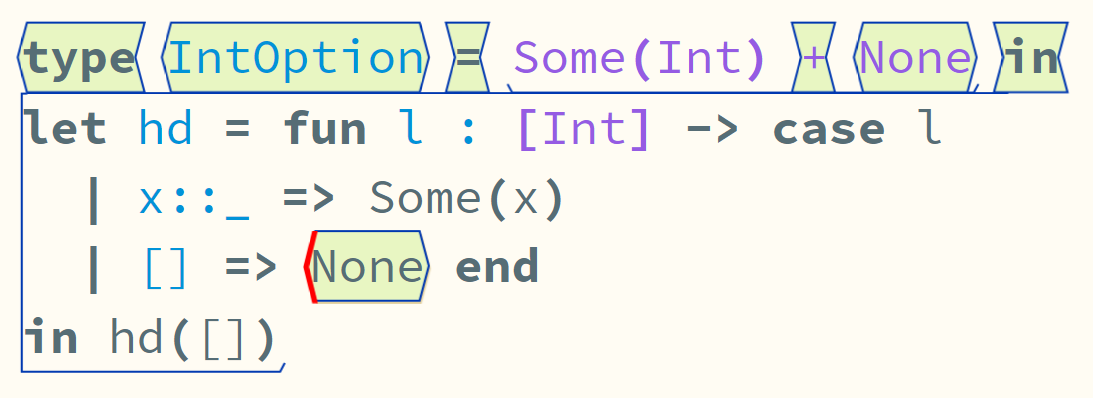
\includegraphics[width=1\textwidth]{Media/Figures/none_syn}
\caption{\code{None} synthesises \code{IntOption} due to it's type definition.}
\end{subfigure}
\begin{subfigure}[t]{0.45\textwidth}
\centering
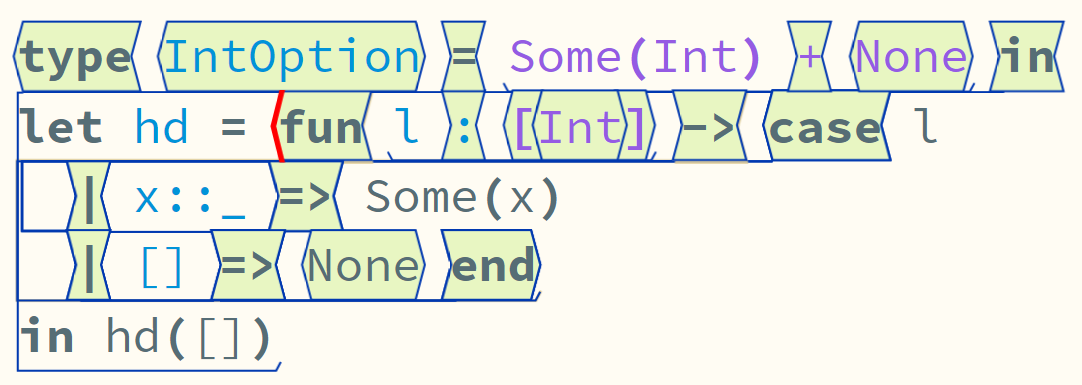
\includegraphics[width=1\textwidth]{Media/Figures/fun_syn}
\caption{The function synthesises \code{[Int]}$\to$ \code{IntOption} due to it's \code{[Int]} annotation and that the match branches synthesis \code{IntOption}. Both branches provide the same type information, only one branch (the last) is highlighted.}
\end{subfigure}
\begin{subfigure}[t]{0.45\textwidth}
\centering
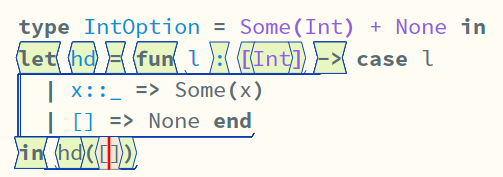
\includegraphics[width=1\textwidth]{Media/Figures/list_ana}
\caption{The list input is expected to be an \code{[Int]} as it is applied to \code{hd} which is a function annotated with input type \code{[Int]}.}
\end{subfigure}
\begin{subfigure}[t]{0.45\textwidth}
\centering
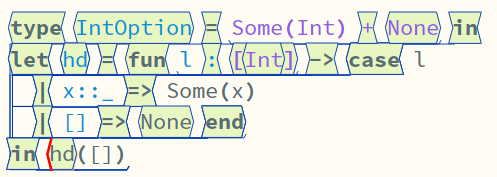
\includegraphics[width=1\textwidth]{Media/Figures/hd_syn}
\caption{The variable usage of \code{hd} synthesises \code{[Int]}$\to$ \code{IntOption} similarly (and also due to the binding).}
\end{subfigure}
\caption{Type Slices}
\label{fig:SliceExamples}
\end{figure}

\section{Cast Slicing Implementation}\label{sec:CastSlicingImplementation}
To implement cast slicing, replace casts between \textit{types} by casts between \textit{type slices}. Type slices are already type-indexed and retain all type information so can be used equivalently.

\subsection{Elaboration}\label{sec:Elaboration}
Cast insertion recursively traverses the unelaborated term, inserting casts to the term's statically determined type as stored in the \code{Info} data-structure and from the type as can be determined directly from the term. 

For example, list literals recursively elaborate it's terms and join their slices, inserting a cast to this join.

Ensuring that all the type slice information from the \code{Info} map is retained and/or reconstructed during elaboration was a meticulous and error-prone process.

\subsection{Cast Transitions}
\Cref{sec:HazelDynamics} gave an intuitive overview of how casts are treated at runtime. Type-indexed slices allows cast slices to be decomposed in exactly the same way. 

However, as Hazel only checks consistency between casts between \textit{ground types}, there are two rules where new\footnote{As opposed to being derived from decomposition.} casts are \textit{inserted} (ITGround, ITExpand). The new types are both created via a \textit{ground matching} relation which takes only the topmost compound constructor, for example ground functions \cref{fig:GroundFunction}. Relevant portions of the appendix are \cref{fig:groundtypes}, \cref{fig:instructions}, \cref{fig:groundmatch}.

As we already store type slices incrementally, the part of the slice which corresponds \textit{only} to the outer type constructor is the outer slice tag.

\begin{figure}
\[\tau_1 \to \tau_2 \match{\text{ground}} \dyn \to \dyn\]
\caption{Ground Matching List}
\label{fig:GroundFunction}
\end{figure}

\subsection{Unboxing}
When a final form (\cref{sec:HazelFinalForms}) has a type, Hazel often needs to extract parts of the term according to the type during evaluation. But due to casts and holes, this is not trivial \cite{LivePatternMatching}.

For example, if a term is a final form of type list, then it could be either:
\begin{itemize}
\item A list literal: \code{[1,2,3]}.
\item A list with casts wrapped around it: \code{[1,2,3]}$\scast{\code{[Int]}}{\code{[}\dyn\code{]}}$.
\item A list cons with indeterminate tail: \code{1::2::?}.
\end{itemize}
Additionally, when the input is not a list at all, it returns \code{DoesNotMatch}, used in pattern matching. 

Unboxing makes use of GADTs to allow for varying output type depending on the type that the final form is being unboxed upon.

\subsubsection{Hazel Unboxing Bug}
While writing the search procedure I found an unboxing \textit{bug} which would always \textit{indeterminately match} a cons with indeterminate tail with \textit{any} list literal pattern (of \textit{any} length), even when it is known that it could never match. For example a list cons \code{1::2::?} represents lists with length $\geq 2$, but even when matching a list literal of length 0 or 1 it would indeterminately match rather than explicitly \textit{not} match. 

Pattern matching checks if each pattern matches the scrutinee with the following behaviour, starting from the first branch:
\begin{itemize}
\item \textit{Branch matches?} Execute the branch.
\item \textit{Branch does not match?} Try the next branch.
\item \textit{Branch indeterminately matches?} Cannot assume the branch doesn't match so must stop evaluation here. The match statement is then indeterminate.
\end{itemize}
\Cref{fig:PatternMatchingBug} demonstrates a concrete example which would get stuck in Hazel, but does \textit{not} need to. I reported and fixed this, with my PR merged into the dev branch.

\begin{figure}[H]
\centering
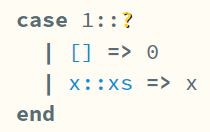
\includegraphics[width=0.25\textwidth]{Media/Figures/unboxing_bug}
\caption{Pattern Matching Bug}
\label{fig:PatternMatchingBug}
\end{figure}


\subsection{User Interface \& Examples}
Type slices within casts can be selected from the evaluation result and displayed. This require reworking some of the dependencies of Hazel's model-view-update architecture to make sure the cursor has access to the code editor cell when inside the evaluation result cell.
\begin{figure}[h]
\centering
\begin{subfigure}{0.45\textwidth}
\centering
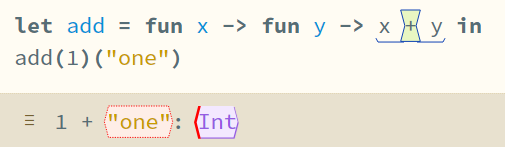
\includegraphics[width=1\textwidth]{Media/Figures/simple_cast_error}
\caption{A simple cast error blaming the plus operator for requiring the integer cast.}
\end{subfigure}
\begin{subfigure}{0.45\textwidth}
\centering
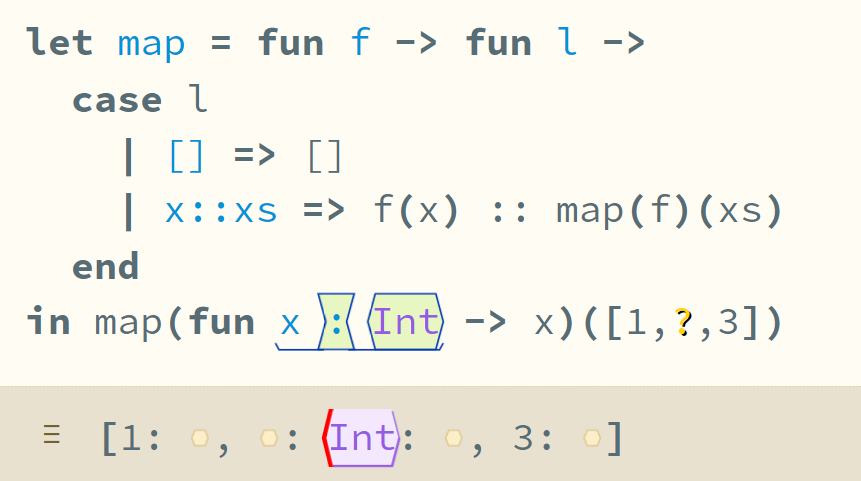
\includegraphics[width=1\textwidth]{Media/Figures/map_cast}
\caption{A hole cast to \code{Int} due to a mapped function annotated with an \code{Int} input.}
\end{subfigure}
\begin{subfigure}{0.65\textwidth}
\centering
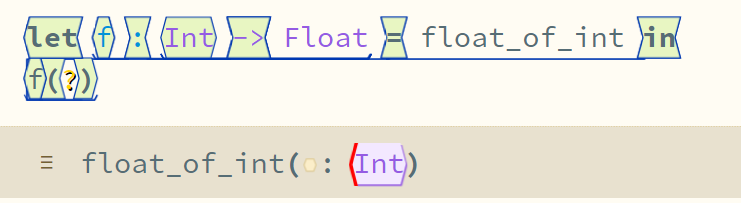
\includegraphics[width=1\textwidth]{Media/Figures/decompose_casts}
\caption{A decomposed cast. The input of the function takes only slice for the argument part \code{Int} of the function type $\code{Int} \to \code{Float}$.}
\end{subfigure}
\caption{Cast Slicing Examples}
\end{figure}
\section{Indeterminate Evaluation}\label{sec:IndetEval}
Dynamic errors include evaluation traces, aiding debugging \cite{TraceVisualisation}. Static type errors lack such traces, as ill-typed programs do not run. Seidel et al. [29] offer an OCaml algorithm using lazy, non-deterministic narrowing of holes to least specific values based on context (e.g., instantiating a hole in + as an integer). 

This section creates a framework for non-deterministic evaluation of indeterminate expressions by lazily performing hole substitutions using type information from dynamic casts. Unlike Seidel, this supports more language features (all of Hazel), any number of inputs (holes), and exhaustive generation of these inputs. Further, it is a general evaluation method, not limited to cast error searches. Specifics relating to cast errors, are covered in \cref{sec:SearchProcedure}.

This section covers the following, answering each question:
\begin{enumerate}
\item[\ref{sec:ResolvingNondeterminism}] How should we resolve the non-determinism in instantiating holes \textit{fairly}? How can the search order be abstracted? Unlike Seidel's approach, my implementation is \textit{fair}: exhaustively considering all possibilities, and allows search methods that avoid (unnecessary) non-termination.
\item[\ref{sec:IndetEvalAlgorithm}] Describes an algorithm for indeterminate evaluation. Is every possibility explored fairly?
\item[\ref{sec:ThreadingState}] How can \textit{per-solution} state be maintained irrespective of evaluation order?
\item[\ref{sec:HoleInstantiation}] Discusses hole instantiation and substitution. What does lazy instantiation actually entail, when exactly should a hole be instantiated? Which hole\footnote{There may be multiple.} should be instantiated in order to continue evaluation to make progress? How should holes be substituted with their narrowed values; the same hole may exist in multiple locations within the expression?
\item[\ref{sec:OneStepEvaluator}] How to use the evaluation abstraction (\cref{sec:EVMODE}) to perform just one evaluation step?
\item[\ref{sec:TypesForHoles}] Finally, I consider Hazel-specific problems. Once we know which hole to instantiate, how can we get it's \textit{expected type}? Hazel's lazy treatment of pushing casts into compound data types means not all such holes will be wrapped directly in casts. Additionally, the case of pattern matching is difficult, allowing holes to be \textit{non-uniformly} cast to \textit{differing types}. How can holes be instantiated in these situations?
\end{enumerate}
As always, a UI is implemented in \cref{sec:UIIndetEval}.

\subsection{Resolving Non-determinism}
\label{sec:ResolvingNondeterminism}
To model infinite non-determinism I create a monadic DSL with an explicitly tree/forest-based representation. The forest model allows for varying low level search traversals. The module type of combinators is in \code{Nondeterminism.Search}; it's underlying parametric type is \code{t('a)} with \code{'a} being the type of the solutions. \Cref{sec:SearchMethods} discusses the actual implementations of this interface, giving four searching procedures.

\subsubsection{Monadic Non-determinism}
\cref{sec:Nondeterminism} described a high level monadic framework for nondeterminism. I extend this with some extra functions:

\begin{itemize}
\item Standard \code{map} and \code{join} functions. Mapping transforms all possible solutions, but does not change if a candidate \textit{is} a solution.
\item \code{once : t('a) => option('a)}, extracts any one solution, if one exists. This can be used to efficiently model \textit{don't care} non-determinism, where if one possibility fails, then we know all others fail also.
\item \code{run : t('a) => Sequence.t('a)} produces a lazy list (Jane Street's \code{Base.Sequence}) of all solutions.
\item \code{guard : bool => t(unit)}, represents success. When chaining binds, if any guard binding fails, then the whole computation fails.
\item \code{ifte : m('a) => ('a => m('b)) => m('b)}. This corresponds to Mercury's interpretation of an if-then-else construct \cite{Mercury}. It is put to good use for computations which explain the failure of the conditional.
\end{itemize}

\subsubsection{Abstracting Search Order: Forest Model}
Typical stream-based models of non-determinism \cite{ListOfSuccess} only admit the possibility of depth-first search (DFS). Stream concatenation provides no way of remembering choice points and backtracking before finishing a computation. 

Instead, monadic non-determinism can be represented by forests \cite{Bunches}. A forest is a list of trees, and can be defined as a monad. Choice, similarly to streams, is performed by concatenating forests. Finally, in order to build tree structure, a \code{wrap} combinator can wrap a forest as a tree whose root leads branches to each tree in the original forest, see \cref{fig:Wrap}.

\begin{figure}[h]
\centering
\begin{subfigure}{0.45\textwidth}
\centering
\[\left[\ 1\quad ; \quad 2 \quad ; \quad 3\ \right]\]
\caption{\code{let x = return(1) <||>} \code{return(2)} \code{         <||> return(3)}}
\end{subfigure}
\begin{subfigure}{0.45\textwidth}
\centering
\[\left[\vcenter{\hbox{\begin{forest}
[$\cdot$ [4] [5]]
\end{forest}}}\right]\]
\caption{\code{let y = wrap(return(4) <||> return(5))}}
\end{subfigure}
\begin{subfigure}{0.45\textwidth}
\centering
\[\left[\vcenter{\hbox{\begin{forest}[$\cdot$ [1] [2] [3]]\end{forest}}} \quad ; \quad\vcenter{\hbox{\begin{forest}[$\cdot$ [4] [5]]\end{forest}}}\right]\]
\caption{\code{let z = wrap(x) <||> y}}
\end{subfigure}
\begin{subfigure}{0.45\textwidth}
\centering
\[\left[\vcenter{\hbox{\begin{forest}[$\cdot$ [$\cdot$ [1] [2] [3]][$\cdot$ [4] [5]]]\end{forest}}}\right]\]
\caption{\code{wrap(z)}}
\end{subfigure}
\caption{Forests Defined Using \code{wrap}}
\label{fig:Wrap}
\end{figure}

Therefore, I extend the DSL with a \code{wrap : t('a) => t('a)} combinator. Here, \code{wrap} is abstract, the underlying implementation does not actually need to use a forest data structure.\footnote{Therefore, DFS can still be efficiently implemented with regular streams.}

These trees can be traversed in various orders, e.g. breadth-first search (BFS)\cite{BFSCombinators}, or bounded DFS. With this in mind, \code{run} now represents performing the search on the tree, returning the solutions in sequence.

In essence, \code{wrap} allows encoding some notion of \textit{cost}\footnote{The depth of the node in the tree.} to solutions, which can then affect the search order.

\subsubsection{Recursive Functions}
As OCaml is strict, defining infinite choices via recursion can lead to non-termination during definition. I define a shorthand lazy application function \code{apply(f, x)} by \code{return(x) >>= f}, represented infix by \code{|>-}. Provided that bind lazily applies \code{f},\footnote{Which it usually does, consider streams as an example.} recursive functions can be written directly resulting in infinite choices without OCaml's strictness leading to infinite recursion.

\subsection{A Non-Deterministic Evaluation Algorithm}
\label{sec:IndetEvalAlgorithm}
This section demonstrates how we can indeterminately evaluation to return all possible values. Demonstrated by \cref{fig:IndetEvalBlock} and with code extract \cref{fig:IndetEval}.

\begin{figure}[h]
\centering
\begin{tikzpicture}[
  node distance=1.8cm and 2.5cm,
  every node/.style={font=\small},
  startstop/.style={rectangle, rounded corners, draw, minimum width=3.5cm, minimum height=1cm, text centered, fill=blue!10},
  process/.style={rectangle, draw, minimum width=3.5cm, minimum height=1cm, text centered, fill=orange!20},
  decision/.style={diamond, draw, aspect=2, text centered, inner sep=1pt, fill=yellow!20},
  arrow/.style={-Latex}
]

% Nodes
\node (start) [startstop] {Bind input to $d$};

\node (classify) [process, below=of start] {\texttt{take\_step}(d)};

\node (isValue) [decision, left=of classify] {Final value?};
\node (isIndet) [decision, below=of classify] {Indeterminate?};
\node (isStep) [decision, below right=of classify] {Can step?};

\node (retVal) [startstop, below=of isValue] {Return $d$ as result};

\node (instantiate) [process, below=of isIndet] {\texttt{instantiate}(d)};

\node (inst1) [process, left= of instantiate] {Instantiation 1};
\node (inst2) [process, below=of inst1] {Instantiation 2};
\node (instN) [below=of inst2] {$\vdots$};

\node (evalNext) [process, below=of isStep] {Step to $d'$};

\node (fail) [startstop, right=of classify] {Exception: \texttt{fail}};

% Arrows
\draw [arrow] (start) -- (classify);

\draw [arrow] (classify) -- (isValue);
\draw [arrow] (classify) -- (isIndet);
\draw [arrow] (classify) -- (isStep);
\draw [arrow] (classify) -- (fail);

\draw [arrow] (isValue) -- node[right] {Yes} (retVal);
\draw [arrow] (isIndet) -- node[right] {Yes} (instantiate);
\draw [arrow] (isStep) -- node[right] {Yes} (evalNext);

% Recursive loop from evalNext to start
\draw [arrow] (evalNext.south) |- ++(4,-1) |- (start.east);

% Instantiate forks
\draw [arrow] (instantiate.west) |- (inst1.east);
\draw [arrow] (instantiate.south) |- (inst2.east);
\draw [arrow] (instantiate.south) |- (instN.east);

% Loop back from each instantiation to start
\draw [arrow] (inst1.west) -- ++(-1,0) |- (start.west);
\draw [arrow] (inst2.west) -- ++(-1,0) |- (start.west);
\draw [arrow] (instN.west) -| ($(inst2.west)+(-1,0)$) |- (start.west);
\end{tikzpicture}
\caption{Block diagram of indeterminate evaluation to values}
\label{fig:IndetEvalBlock}
\end{figure}

Instantiation is implemented by a \textit{non-deterministic} function \code{instantiate}, discussed in detail in \cref{sec:HoleInstantiation}: \[\code{Instantiation.instantiate : Exp.t => m(Exp.t)}\]

Classifying a term $d$, into values, indeterminate terms, and expressions with a possible step is done by a (deterministic) function \code{take_step}, discussed in \cref{sec:OneStepEvaluator}: \[\code{OneStepEvaluator.take_step : Exp.t => TryStep.t}\] 

To ensure that the search tree has finite branching factor, possibly infinite choices must be wrapped, e.g. evaluation steps. To allow for multiple searching methods, the algorithm is placed within a \textit{functor}, which takes a searching method, \code{S : Search}.

\begin{figure}[h]
\begin{minted}{reason}
module Make = (S: Search) => {
  module Instantiation = Instantiation.Make(S);
  open S;
  open S.Infix;
  
  let rec values = (d: DHExp.t) : S.t(DHExp.t) => {
    let step = OneStepEvaluator.take_step(d);
    switch (step) {
    | BoxedValue => return(d)
    | Indet => 
      d |>- Instantiation.instantiate
        >>- values;
    | Step(d') => wrap(d' |>- values);
    | exception (EvaluatorError.Exception(_)) => fail
    };
  };
};
\end{minted}
\caption{Indeterminate Evaluation to Values}
\label{fig:IndetEval}
\end{figure} 

\subsection{Threading Evaluation State}
In order to track statistics for use in the evaluation, state must be threaded through indeterminate evaluation. State tracked includes, on a \textit{per-solution} basis:
\begin{itemize}
\item Trace length.
\item Number of and size of instantiations performed.
\end{itemize}

So instead of threading only the solutions, \code{DHExp.t}, I also thread the state, \\\code{(DHExp.t, IndetEvaluatorState.t)}, updating according depending on the branch taken.

Additionally, Hazel evaluates expressions in an global environment (\code{env : Environment.t}) which must also be passed down, but does not change after performing a step.

\subsection{Hole Instantiation \& Substitution}\label{sec:HoleInstantiation}
There are three key problems to solve in order to instantiate terms.

\subsubsection{Choosing which Hole to Instantiate}
\label{sec:ChooseHole}
An indeterminate term may contain \textit{multiple} holes or even \textit{no} holes. Which hole needs to be instantiated in order to \textit{make progress}?

When attempting to evaluate the indeterminate term some transitions rules require a sub-term to be concrete (e.g. a function during application). We chose to instantiate the hole that blocks the \textit{first} blocked transition rule. If latter holes were instantiated, the term might \textit{still} be unevaluable due to this first hole.

This is implemented using Hazel's evaluator abstraction (\code{EV_MODE}), separating this logic from the transition semantics. Therefore, hole choice logic will automatically update to any future changes in the transition semantics.

\subsubsection{Synthesising Terms for Types}
Suppose we know which hole to instantiate and to which type (\cref{sec:TypesForHoles}). How do we refine these holes fairly and lazily, to the \textit{least specific} value that allows evaluation to continue?

Base types must be instantiated directly to their (possibly infinite set of) values, for example:
\paragraph{Booleans:} \code{return(true) <||> return(false)}.
\paragraph{Integers:} A recursive definition using lazy application \code{|>-}, see \cref{fig:Integers}:
\begin{figure}[h]
\begin{minted}{reason}
let rec ints_from = n => return(n) <||> wrap(n + 1 |>- ints_from)
let nats = ints_from(0)
let negs = ints_from(1) >>| n => -n
let ints = nats <||> wrap(negs) 
\end{minted}
\begin{subfigure}{0.45\textwidth}
\centering
\[\left[\ n \quad ; \quad \vcenter{\hbox{\begin{forest}
[$\cdot$ [$n+1$] [$\cdot$ [$n + 2$] [$\cdot$ [$n+3$] [...]]]]
\end{forest}}}\right]\]
\caption{\code{ints_from(n)}}
\end{subfigure}
\begin{subfigure}{0.45\textwidth}
\centering
\[\left[\ 0 \quad ; \quad \vcenter{\hbox{\begin{forest}
[$\cdot$ [$1$] [$\cdot$ [$2$] [$\cdot$ [$3$] [...]]]]
\end{forest}}} \quad ; \quad \vcenter{\hbox{\begin{forest}
[$\cdot$ [$-1$] [$\cdot$ [$-2$] [$\cdot$ [$-3$] [...]]]]
\end{forest}}}\right]\]
\caption{\code{ints}}
\end{subfigure}
\caption{Enumerating Integers}
\label{fig:Integers}
\end{figure}
 
\paragraph{Strings:} A string is either \textit{empty} or is a string with a first character from a finite set. We can recursively wrap all strings, prefixed by each character. See \cref{fig:Strings}:
\begin{figure}[h]
\begin{minted}{reason}
let chars = // Every single letter string considered
let rec strings = () => return("") 
  <||> wrap(chars >>= chr => 
            (() |>- strings) >>- str => 
            chr ++ str)) 
\end{minted}
\caption{Enumerating Strings}
\label{fig:Strings}
\end{figure}
\

Other types are \textit{inductive}, these can be represented indirectly by lazily instantiating only their \textit{outermost} constructor: 
 
\paragraph{Lists:} A list is either the empty list, $[\ ]$ or a cons $\dyn_1 :: \dyn_2$. Note that, to retain the correct dynamic type information, $\dyn_2$ must be cast back to the list type. 
\paragraph{Sum Types:} Enumerate each of the sum's constructors with their least specific value.
\paragraph{Functions:} Constant functions have least specific values $\lambda \_.\ \dyn$. The function may then be applied to any value, and it's result synthesised after application. This can synthesise any return value, hence errors in the usage of the function will be detected. But, if the \textit{input} has an erroneous type but is uncaught as the function is dynamic, potential errors arising from this cannot be found.\footnote{This can occur in dynamic functions with inconsistent branches. But this is extremely rare, and can be fixed for most cases by generating the identity function where function hole's expected type allow.} Extensions to program synthesis (\cref{sec:LogicProgramming}) would require more sophisticated function instantiation.


\subsubsection{Maintaining Correct Casts}
Every hole has a dynamic type at runtime. Therefore, that hole's context \textit{expects} it to have the dynamic type. Therefore, we must cast every instantiation back to the dynamic type.

\subsubsection{Substituting Holes}\label{sec:HoleSubstitutionImplementation}
Holes can be bound to variables in the execution environment, and may also be duplicated, before they are required to be instantiated, see \cref{fig:HoleDuplication}. Therefore, instantiations must be substituted for every occurrence of the same hole.

\begin{figure}[h]
\centering
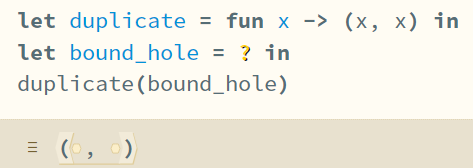
\includegraphics[width=0.4\textwidth]{Media/Figures/duplicate_hole}
\caption{Duplicated Holes}
\label{fig:HoleDuplication}
\end{figure}

Consistent hole substitution was described as part of the Hazel calculus \cref{sec:HoleSubstitution}. Unexpectedly, the main Hazel branch did not yet implement it. A full implementation of metavariables and delayed closures is complex. Therefore, as hole closures are not required for hole instantiation,\footnote{Currently, there is no need to instantiate to a variable reference.} I instead use the existing term ids to represent metavariables, and ensure these ids are maintained and propagated correctly throughout statics, elaboration, and evaluation.\footnote{A huge portion of the code-base required checks.}

We can substitute terms for every hole with the given ID throughout the entire expressions. Substitutions within closures \textit{include} eagerly evaluating the resulting binding to ensure the invariant that closures bind variables to values. 

\subsection{One Step Evaluator}\label{sec:OneStepEvaluator}
The step evaluator uses the evaluation abstraction to create an \textit{evaluation context} from a term, to return:
\begin{itemize}
\item An evaluation context, with a \textit{mark} inserted in place of the sub-term which is evaluated according to the transition rules.
\item The environment under which the sub-term is evaluated.
\item The kind of rule that was used (e.g. substitution, addition, etc.).
\end{itemize}

This information allows indeterminate evaluation methods to treat different steps differently. For example one might wish to return only the substitution steps, to produce a compressed execution trace.

\subsection{Determining the Types for Holes}
\label{sec:TypesForHoles}
If we know which hole to instantiate, how do we know which type to instantiate it to?

For efficiency, my implementation both determines \textit{which hole}, and it's \textit{type information} during the same pass.

\subsubsection{Directly from Casts}
Most of the time, a hole is directly surrounded by a cast, whose type information can be used to perform an instantiation.

\subsubsection{Cast Laziness}\label{sec:CastLaziness}
However, this is \textit{not} always the case. For efficiency reasons, Hazel treats casts over compound data-types lazily, e.g. casts around tuples will only by pushed inside upon usage of a component of the tuple.

Treating casts eagerly is a significant change to the Hazel semantics, so was opted against. \Cref{sec:EvalCastLaziness} discusses the consequence of this choice. 


\subsubsection{Pattern Matching}
\label{sec:PatternMatching}
Does a hole even have only one possible type?

The introduction of (dynamic) pattern matching actually allows terms to be matched against \textit{non-uniform} types if the scrutinee is dynamic. In \cref{fig:DynamicPatternMatching}, if \code{term} is an integer 0 then it returns 0, but if it's the string "one" then it returns 1. Hence instantiating \code{code} to either an int or string might allow progress.

\begin{figure}[h]
let term : ? =   in
case term 
  | x::xs => x
  | 0 => 0
| "one" => 1 end 
\label{fig:DynamicPatternMatching}
\end{figure}

Hazel implements this by placing casts on the \textit{branches}, rather than the scrutinee. Therefore, we can collect each of these possible types from the casts, and wrap them around the scrutinee, continuing evaluation accordingly.


\begin{figure}
Show how indeterminate matches cause a list to try increasing lengths by repeatedly instantiating it's tail...
\caption{Instantiating a Scrutinee}
\end{figure}

\subsubsection{Extended Match Expression Instantiation (Pattern Instantiation)}
\label{sec:ExtendedPatternMatching}
An interesting extension was partially implemented which improves code coverage and additionally detects errors within patterns. 

It instantiates holes in a match expression according also to the \textit{structure} of each pattern, allowing the instantiation to prioritise searching along each branch. We instantiate the scrutinee with the least specific versions which match the patterns on each branch, e.g. \code{?::?} for \code{x::xs}. However, sometimes this instantiation is not specific enough to explicitly not match with previous statements, hence getting stuck. Proposed solutions can be found in \cref{sec:extendedmatching}.

\subsection{User Interface}\label{sec:UIIndetEval}
The default evaluation method returns every possible indeterminate or concrete values. The possibilities can be cycled through via some arrows buttons.

\section{Search Procedure}\label{sec:SearchProcedure}
Now that an framework for indeterminate evaluation has been specified, the following problems can be addressed:
\begin{itemize}
\item[\ref{AbstractSearch}] How can indeterminate evaluation be abstracted into a generic search procedure?
\item[\ref{CastFailureDetection}] What exactly are cast errors? How can they be detected? Which ones are actually \textit{relevant}, causing evaluation to get stuck?\footnote{Some cast errors are known, e.g. from static type checking, but don't actually relate to the evaluation path.}
\item[\ref{SearchMethods}] How can different search methods be implemented: DFS, BFS, Iterative deepening DFS? 
\end{itemize}

\subsection{Abstract Indeterminate Evaluation}
\label{sec:AbstractSearch}
By making the search procedure take a higher-order \code{logic : Exp.t => TryStep.t => S.t('a)} function, which takes the an input expression $d$ and it's class (value, indet, step possible), and returns nondeterministic results of type \code{'a}.

This allows defining search procedures returning other types, for example, the integer \textit{size} of values. Or those concerning specific types of expressions, for example only those with cast errors. 

Additionally, an `expert' search abstract is given, which also allows the remaining search space to be defined. This allows, for example, customising the instantiation and evaluation methods.

\subsection{Detecting Relevant Cast Errors}
\label{sec:CastFailureDetection}
To search for cast errors, we must first define what one is. A reasonable definition is terms which contain \textit{cast failures}, in Hazel these are casts between \textit{inconsistent ground types}. However, this has some issues:

\paragraph{Multiple Cast Failures:} Terms may have multiple cast failures, some of which discovered during static type checking and inserted via elaboration. The aim of this project was to allow give dynamic traces \textit{explaining} a static type error. Clearly these failure must be ignored.

Additionally, the procedure has usage searching for errors in dynamic code. Situations which cause cast errors which don't actually stop evaluation should also be ignored. For example expressions which cannot be statically typed, but are safe, are within this class: \code{if true then "str" else 0}

Therefore, we consider only the casts which are \textit{causing} a term to be indeterminate (therefore getting stuck), this is implemented similarly to choosing which hole to instantiate (\cref{sec:ChooseHole}).

\paragraph{Cast Laziness}
\label{sec:SearchCastLaziness}
Only casts between \textit{ground} types are checked for consistency. Due to cast laziness (\cref{sec:CastLaziness}), some are cast between inconsistent types, but \textit{not} placed within a \textit{cast failure}.

This can be fixed by performing eager cast transitions before checking for cast errors, or eagerly treating casts during indeterminate evaluation. However, it could be argued that this \textit{should not} constitute a cast error, after all, the part of the compound type with the error is yet to actually be \textit{used}.

\paragraph{Dynamic Match Statements:} When matching dynamically on values with different types, the instantiations wrap the scrutinee in casts to each type. If any of these casts failed, they should not count as witnesses, as they were introduced entirely by the instantiation procedure. 

\subsection{Explaining Cast Errors}
\label{sec:StaticCastError}
A static type error will place a term inside a cast error during elaboration. The id of this error can be tracked, and if it is the one at fault, associated with the static error. Additionally, the type slice enforcing the cast is tracked via cast slicing, and may be displayed as usual.

\subsection{Searching Methods}\label{sec:SearchMethods}
\textbf{Note: Should remove fair choice and conjunction, in favour of it just being an interleaved search method (see interleaved DFS below)}

I implement \textit{four} different search methods, implementing the non-determinism signature specified in \cref{sec:ResolvingNondeterminism}.

\subsubsection{Depth First Search}
As mentioned previously \textbf{(REF)}, modelling lazy sequences by streams is a typical method, and implementing choice and conjunction via appending leads to depth-first search. In which case, \code{wrap} is just the identity function.

\begin{figure}
Show how streams \& append represent depth first search
\caption{Depth First Search as Streams}
\end{figure}

\subsubsection{Breadth First Search}
Breadth first search needs to take specific account of the tree structure. Sequences of bags\footnote{Lists, but where ordering doesn't matter.} can be used to represent solutions at each \textit{level} of the tree \cite{BFSCombinators}. Therefore, forcing each element of the stream gives the solutions at successive depths, i.e. iterating through these bags returns the solutions in a breadth first order.

Failure is the empty sequence as before, return injects a solution into a tree giving the solution in the first level. 

Choice can be represented lazily merging of each level of the tree. The merged tree would produce all solutions of the first level of each choice at the same time, as the new first level. This is associative as required, when ignoring the ordering of each level, as is done with bags. 

\begin{figure}[h]
Merge trees, show that it maintains BFS.
\caption{Breadth First Choice}
\end{figure}

Wrapping a tree pushes every solution one level down in the tree, corresponding to prepending with the empty list. Essentially, this adds one cost to every solution.

For a bag \code{b} of elements \code{x1}, \code{x1} $\dots$, \code{xn}. The tree which produces these solutions in the first level, $[b]$\footnote{Using list notation also for sequences}, is equivalent to \code{return(x1) <||> return(x2) <||> ... <||> return(xn)}.

A tree \code{b :: bs} is equivalent to \code{[b] <||> [] :: wrap(bs)}, and by the above, also equivalent to \code{return(x1) <||> ... <||> return(xn) <||> wrap(bs)}.

Therefore, as conjunction distributes over choice, and return is a left unit of conjunction then:
\[\code{b :: bs >>= f     =    f(x1) <||> ... <||> f(xn) <||> wrap(bs >>= f)}\]
Additionally, another law for non-determinism \code{fail >>= f = fail}, completes a recursive definition for bind.

As mapping and choice are associative, we get that conjunction is also. Additionally, it satisfies all the remaining monad and non-determinism laws. 

However, as \code{f} is mapped to the entire bag \code{b}, it is difficult to maintain laziness in OCaml. We need partial applications for f... \textbf{TODO - can't actually work out how to do this in OCaml?!?!}

\subsubsection{Iterative Deepening Depth First Search}
While breadth first search is fair, avoiding non-termination (for finite branching factor), it has \textit{exponential} space complexity in the depth of the level being explored \cite{NorvigAI}. When binding a function \code{f}, it gets lazily and \textit{partially} instantiated at node of each level, tracking these partial instantiations is what causes the exponential complexity.

\begin{figure}

\caption{Monadic BFS Requires Exponential Space}
\end{figure}

In comparison, depth first search only requires space linear in the depth explored, that is, the number of choices encountered before reaching a certain depth.

The use of iterative deepening, successive depth-bounded depth first searches, retains low space complexity of DFS while also avoiding non-termination (due to the depth bound). However, upper parts of the search tree will be repeatedly explored, but this does not reduce the already exponential time complexity of the search for branching factor greater than 1. But, the deterministic evaluation part does have a branching factor of 1, so it may be the case that the recalculation has a significant impact\textbf{(Ref evaluation)}. 

To represent iterative deepening \cite{SearchAlgebra}, we can use functions \code{int => list(('a, int))}, calculating every\footnote{Again, relying on finite branching factor.} solution found within an integer depth bound \code{d}, alongside it's remaining depth budget \code{r}. Tracking the remaining depth budget simplifies \code{bind} and allows only solutions on the fringe (zero budget) to be output upon each iteration, so the same solution will not appear twice.

Then, \code{return} represents a single solution with unused depth budget, \code{return(x)  =  (d => [(x, d)])}. \code{fail} gives the empty list \code{fail  =  d => []}. Choice appends all solutions at any given depth bound \code{m <||> n  =  d => m(d) @ n(d)}. Binding, \code{m >>= f} takes solutions in \code{m} who have depth budget to use, and applies \code{f} and calculates all solutions from \code{f} using the remaining budget, concatenating these results to form a single list.

Then \code{wrap(m)} (the forest \code{m} wrapped up as a single tree) has solutions at depth incremented by 1, and none at depth 0: \code{wrap(m)(0) = []} and \code{wrap(m)(bound) = p(bound - 1)}.

I implement this as a functor, with a custom bound incrementing function \code{inc : bound => bound} and initial bound \code{init : bound}. Then \code{run} will   search to depth \code{init}, produce all solutions, then search to depth \code{inc(init)} and produce all solutions with remaining depth budget \code{inc(init) - init}, other solution must have already been produced last iteration.

\begin{figure}
\begin{minted}{reason}
((m >>= f) >>= g)(bound)
= m(bound) 
  |> map((x, rem_bound) => f(x, rem_bound))
  |> concat
  |> map((y, rem_bound2) => g(y, rem_bound2))
  |> concat
\end{minted}
Vs.
\begin{minted}{reason}
(m >>= (x => f(x) >>= g))(bound)
= m(bound)
  |> map((x, rem_bound) => rem_bound |> (f(x) >>= g))
  |> concat
= m(bound)
  |> map((x, rem_bound) => rem_bound |> (f(x) 
  |> map((y, rem_bound2) => g(y, rem_bound2)) 
  |> concat))
  |> concat
= m(bound)
  |> map((x, rem_bound) => f(x, rem_bound) 
  |> map((y, rem_bound2) => g(y, rem_bound2))
  |> concat)
  |> concat
= m(bound)
  |> map((x, rem_bound) => f(x, rem_bound)) 
  |> concat
  |> map((y, rem_bound2) => g(y, rem_bound2))
  |> concat
\end{minted}
\caption{Associativity of Iterative DFS \code{bind}}
\end{figure}

\subsubsection{Interleaved Streams}
\textbf{TODO: split code into a new option, remove fair operators, move fair conjunction and chocie section to here.}

The use of streams, but with fair choice and conjunction via interleaved ordering ensures termination for every solution. This has the advantage of working even for trees with infinite branching factor. However, interleaving has a linear space complexity, leading to the undesirable exponential space complexity as with breadth-first search.

\code{wrap} for this is the identity, same as DFS.

\subsection{User Interface}

\section{Repository Overview}
\subsection{Branches}
Up to date with dev branch up to \textbf{DATE}

\subsection{Hazel Architecture}



